\documentclass{beamer}

\usepackage[utf8]{inputenc}
\usepackage[spanish]{babel}
\usepackage{graphicx}

\xdefinecolor{rojito}{rgb}{1,0.3,0.3}
\xdefinecolor{oliva}{cmyk}{0.64,0,0.95,0.4}
\xdefinecolor{minaranja}{rgb}{0.94,0.48,0.2}

\usetheme{Madrid}
\usecolortheme[named=rojito]{structure}

\title[Computación Cuántica]{Introducción a la Computación Cuántica}
\author{Luis Aguirre \& Javier Pellejero}
\institute[UCM]{Universidad Complutense de Madrid\\ Facultad de Informática}

\newcommand{\filados}[2]{ \left. \begin{array}{c}	#1 \\	#2	 \end{array} \right. }
\newcommand{\filacuatro}[4]{ \left. \begin{array}{c}#1\\#2\\#3\\#4	\end{array} \right.}
\newcommand{\base}[1]{|#1\rangle}
\newcommand{\lbase}[1]{\langle#1|}
\newcommand{\dotproduct}[2]{\langle#1|#2\rangle}
\newcommand{\tensor}[2]{|#1\rangle\langle#2|}
\newcommand{\baseup}{\mid\uparrow\rangle}
\newcommand{\baseright}{\mid\rightarrow\rangle}
\newcommand{\baseupright}{\mid\nearrow\rangle}
\newcommand{\baseupleft}{\mid\nwarrow\rangle}
\newcommand{\transpose}[1]{#1 ^\dag}
\newcommand{\complex}{\mathbb{C}}
\newcommand{\puertai}{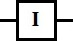
\includegraphics[scale=0.8]{imagenes/puertai}}
\newcommand{\puertax}{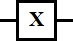
\includegraphics[scale=0.8]{imagenes/puertax}}
\newcommand{\puertay}{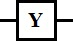
\includegraphics[scale=0.8]{imagenes/puertay}}
\newcommand{\puertaz}{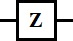
\includegraphics[scale=0.8]{imagenes/puertaz}}
\newcommand{\puertah}{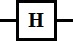
\includegraphics[scale=0.8]{imagenes/puertah}}
\newcommand{\puertacnot}{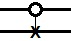
\includegraphics[scale=0.8]{imagenes/puertacnot}}
\newcommand{\eprpair}{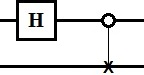
\includegraphics[scale=0.8]{imagenes/eprpair}}
\newcommand{\cnot}{C_{\mathrm{not}}}

\begin{document}

\begin{frame}
	\titlepage
	\begin{center} Doble Grado en Matemáticas e Ingeniería Informática\end{center}
\end{frame}

\begin{frame}
\frametitle{Índice}
	\tableofcontents
\end{frame}

\section{Una primera aproximación mediante la polarización de fotones}

\begin{frame}
	\frametitle{Una aproximación mediante la polarización de fotones}
	Tenemos tres filtros de polarización de luz:
	\begin{itemize}
		\item \textbf{Filtro A:} de polarización horizontal $\rightarrow$.
		\item \textbf{Filtro B:} de polarización diagonal $\nearrow$.
		\item \textbf{Filtro C:} de polarización vertical $\uparrow$.
	\end{itemize}
\end{frame}

\begin{frame}
	\frametitle{Una aproximación mediante la polarización de fotones}
	Colocamos el \textbf{filtro A} tras una fuente de luz y vemos que los rayos han quedado polarizados horizontalmente con una intensidad de aproximadamente el 50 \%.
	\begin{center}
	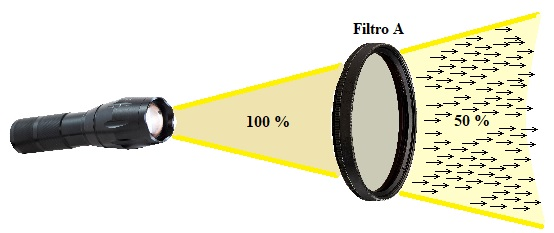
\includegraphics[scale=0.6]{imagenes/polarizacion1}\\
	Experimento 1.
	\end{center}
	Nótese que el filtro no sólo deja pasar a los rayos previamente polarizados horizontalmente. Debido a la aleatoriedad de la polarización de la fuente, que la mitad de los rayos tuviera dicha polarización exacta sería imposible.		
\end{frame}

\begin{frame}
	\frametitle{Una aproximación mediante la polarización de fotones}
	Ahora, tras el filtro A, colocamos el \textbf{filtro C}. Podemos observar que la luz que traspasa ambos filtros es nula.
	\begin{center}
	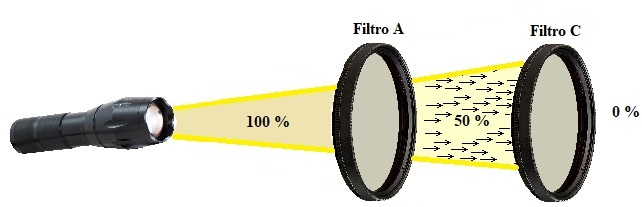
\includegraphics[scale=0.6]{imagenes/polarizacion2}\\
	Experimento 2.
	\end{center}		
\end{frame}

\begin{frame}
	\frametitle{Una aproximación mediante la polarización de fotones}
	Sin embargo, si ahora colocamos el \textbf{filtro B} entre ambas, sí que obtenemos luz 		tras traspasar todos los filtros, aunque sólo $\dfrac{1}{8}$ parte del original.
	\begin{center}
	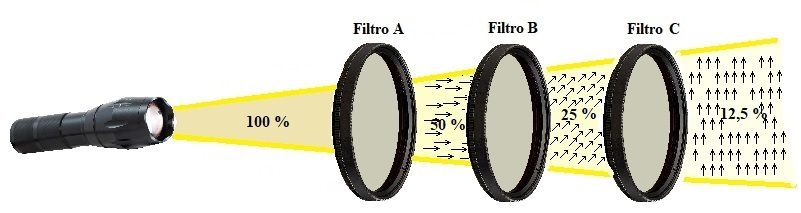
\includegraphics[scale=0.55]{imagenes/polarizacion3}\\
	Experimento 3.
	\end{center}
\end{frame}

\begin{frame}
	\frametitle{Una aproximación mediante la polarización de fotones}
	Conclusiones:
	\begin{itemize}
	\item Cada filtro realiza una ``medida'' que \textbf{cambia} la polarización de cada fotón. 
	\item Sean las bases $\baseup$ y $\baseright$, podemos denotar la polarización de un rayo cualquiera como $\base\psi =\ a\baseup\ +\ b\baseright$ con $a,b \in\complex$ y $|a|^2+|b|^2=1.$
	\item La medición de un rayo en esas bases obtendrá $\baseup$ con una probabilidad de $a^2$ o $\baseright$ con una probabilidad de $b^2$.
	\item Debido a la aleatoriedad inicial, aproximadamente un 50\% de los rayos serán reflejados (medición $\baseup$) y el resto los atravesará ($\baseright$).
	\item Tras la medición en el filtro A, todos los rayos tendrán el estado $\baseright = 0\baseup + 1\baseright$. Así, el filtro C refleja todos los rayos pues la probabilidad de medir $\baseup$ es cero.
	\end{itemize}
\end{frame}

\begin{frame}
	\frametitle{Una aproximación mediante la polarización de fotones}
	\begin{itemize}
	\item Colocando el filtro B cambiamos de base a $\{\baseupright, \baseupleft\}=$ $=\{\dfrac{1}{\sqrt{2}}(\baseup + \baseright), \dfrac{1}{\sqrt{2}}(\baseup - \baseright)\}$.
	\item Véase que $\baseright = \dfrac{1}{\sqrt{2}}(\baseupright - \baseupleft)$ y $\baseup = \dfrac{1}{\sqrt{2}}(\baseupright + \baseupleft)$.
	\item Así, la posibilidad de que al medir $\baseupright$ en el filtro B es de $\left(\dfrac{1}{\sqrt{2}}\right)^2=$ $=\dfrac{1}{2}$ y el estado de los rayos se proyectará en $\baseupright=\dfrac{1}{\sqrt{2}}(\baseup + \baseright)$.
	\item Por tanto, ahora sí podrán traspasar el filtro C, de nuevo con probabilidad $\dfrac{1}{2}$. Como cada filtro ha reflejado el 50\% de los rayos que le han llegado, sólo una octava parte ha traspasado los tres y tendrán estado $\baseup$.
	\end{itemize}
\end{frame}

\section{Estados cuánticos y notación}

\begin{frame}
	\frametitle{Estados cuánticos y notación}
	Sean $\base{x}$ y $\base{y}$ estados cuánticos.
	\begin{itemize}
	\item Denotamos $\lbase{x}$ como el traspuesto de $\base{x}$.
	\item Denotamos el producto escalar como $\lbase{x}\base{y}$ o simplemente $\dotproduct{x}{y}$.
	\item Denotamos el producto tensorial como $\tensor x y$.
	\end{itemize}
	
	\begin{block}{Ejemplo}
	Supongamos que trabajamos en la base $\{(1,0)^T, (0,1)^T\}$ que denotamos como $\{\base{0},\base{1}\}$.
	\begin{itemize}
	\item $\dotproduct 0 0 =1$ y $\dotproduct 0 1 =0$
	\item $\tensor 0 1 = \left({\begin{array}{c}   1\\0\\ \end{array} } \right)\left({\begin{array}{cc}   0 & 1\\ \end{array} } \right)=\left({\begin{array}{cc}   0 & 1\\ 0&0\\ \end{array} } \right)$
	\item Por tanto, $\tensor 0 1$ convierte $\base 1$ a $\base 0$ y $\base 0$ a $(0,0)^T$.
	\end{itemize}
	\end{block}
\end{frame}


\begin{frame}
	\frametitle{Estados cuánticos y notación}
	\begin{block}{Definición}
	Definimos \textbf{bit cuántico} o \textbf{qubit} como un vector unitario complejo de dos dimensiones en una base ortonormal previamente fijada $\base 0$ y $\base 1$ que representa la  superposición de dos estados. Lo representamos como $a\base0+b\base1$ con $a,b\in\complex$ tal que $|a|^2+|b|^2=1$.
	\end{block}
	¿Qué pasa cuando tenemos múltiples qubit?
	\begin{itemize}
	\item En espacios clásicos, si V y W son espacios clásicos con bases $\{\mathrm{v}_1,\mathrm{v}_2\}$ y $\{\mathrm{w}_1,\mathrm{w}_2\}$ respectivamente, la ``unión'' de esos dos subespacios viene dada por el \textbf{producto cartesiano} de ambos que toma como base la unión de las anteriores $\{\mathrm{v}_1,\mathrm{v}_2,\mathrm{w}_1,\mathrm{w}_2\}$. Se cumple que la Dim(V$\times$W) = Dim(V) + Dim(W).
	\item Sin embargo, en espacios cuánticos, dicha ``unión'' viene dada por el \textbf{producto tensorial} que produce $\{\mathrm{v}_1\otimes\mathrm{w}_1,\mathrm{v}_1\otimes\mathrm{w}_2, \mathrm{v}_2\otimes\mathrm{w}_1,\mathrm{v}_2\otimes\mathrm{w}_2\}$.
	\end{itemize}
\end{frame}


\begin{frame}
	\frametitle{Estados cuánticos y notación}
	\begin{itemize}
	\item Así para dos qubits que tienen bases $\{\base0,\base1\}$ se genera $\{\base0\otimes\base0, \base0\otimes\base1, \base1\otimes\base0,\base1\otimes\base1\}$ o $\{\base{00},\base{01},\base{10},\base{11}\}$.
	\item Para 3 bits tendríamos $\{\base{000},\base{001},\base{010},\base{011},\base{100},\base{101},\base{110},\base{111}\}$.
	\item Se verifica así que Dim(V$\otimes$W) = Dim(V) $\times$ Dim(W).
	\item Sin embargo, no podemos alcanzar algunos estados en términos de sus componentes por separado. Por ejemplo $\base{00}+\base{11}$. Deberían existir $(a_1\base0+b_1\base1)\otimes(a_2\base0+b_2\base1)=$ $=a_1a_2\base{00}+a_1b_2\base{01}+b_1a_2\base{10}+b_1b_2\base{11}\neq\base{00}+\base{11}$ Puesto que $a_1$ o $b_2$ o ambos debe ser cero. 
	\end{itemize}
\end{frame}

\begin{frame}
	\frametitle{Estados cuánticos y notación}
	\begin{block}{Ejemplo. Medida en un sistema de 2 qubits.}
	Midamos el primer bit en la base $\{\base0,\base1\}$. Sea el estado $a\base{00}+b\base{01}+c\base{10}+d\base{11}$ con $|a|^2+|b|^2+|c|^2+|d|^2=1$. 
	\end{block}
	\begin{itemize}
	\item Lo reescribimos como $\base0(a\base0+b\base1)+\base1(c\base0+d\base1)=$ $=u\base0\otimes(\frac{a}{u}\base0+\frac{b}{u}\base1) + v\base0\otimes(\frac{c}{v}\base0+\frac{d}{v}\base1)$ con $\filados{u=\sqrt{|a|^2+|b|^2}}{v=\sqrt{|c|^2+|d|^2}}$.
	\item Nótese que $\frac{a}{u}\base0+\frac{b}{u}\base1$ y $\frac{c}{v}\base0+\frac{d}{v}\base1$ son vectores unitarios.
	\item Así la medida del primer qubit arrojará $\base0$ con probabilidad $u^2$ y proyectará el estado $\base0\otimes(\frac{a}{u}\base0+\frac{b}{u}\base1)$.
	\item O arrojará $\base1$ con probabilidad $v^2$ proyectando el estado $\base1\otimes(\frac{c}{u}\base0+\frac{d}{u}\base1)$.
	\end{itemize}
\end{frame}

\section{Paradoja EPR}

\begin{frame}
	\frametitle{Paradoja EPR}
	\begin{itemize}
	\item Experimento realizado por Einstein, Podolsky y Rosen en el que proponían la existencia de dos partículas entrelazadas en el siguiente estado: $\dfrac{1}{\sqrt{2}} \base{00} + 		 		\dfrac{1}{\sqrt{2}} \base{11}$. Mandamos una de las partículas a Alice y la otra a Bob, que pueden estar a una distancia arbitraria. 
	\item Si Alicia realiza una ``medida'' y observa $\base0$, eso implicará que el estado de ambas partículas es  $\base {00}$ y por tanto si Bob ``midiese'' también observaría $\base0$. 		De manera similar ocurriría si Alice hubiese observado $\base1$.
	\item Por tanto, el cambio en el estado cuántico de las partículas se produce de manera instantánea independientemente de la distancia entre Alice y Bob. Es decir, se podrían 				comunicar más rápido que la velocidad de la luz. 
	\end{itemize}
\end{frame}

\begin{frame}
	\frametitle{Paradoja EPR}
	A consecuencia de ello, se propusieron dos modelos para tratar de entender el entrelazamiento entre partículas:
	\begin{itemize}
	\item El primero proponía la existencia de una variable oculta que determinaba completament	el estado: $\base {00}$ o $\base {11}$. Sin embargo, esta teoría fue descartada a traves de 		experimentos reales.
	\item La segunda proponía la existencia de dos observadores, uno que veía ``medir'' a Alice primero, y otro que veía a Bob ``medir'' antes. 
	Según la teoría de la relatividad el comportamiento físico debe ser independiente del observador. Por tanto el experimento debe 	poder explicarse tanto si Bob ``mide'' y afecta a la 				``medida'' de Alicia, como al contrario. Es decir, solo podemos constatar que Alice y Bob observan el mismo comportamiento aleatorio, y no que se hayan comunicado más rápido que la velocidad de la luz.
	
	\end{itemize}
\end{frame}

\section{Operaciones en sistemas cuánticos: Puertas cuánticas}

\begin{frame}
	\frametitle{Operaciones en sistemas cuánticos: Puertas cuánticas}
	\begin{block}{Definición}
	Definimos \textbf{puerta cuántica} como una transformación en el espacio de los vectores complejos. Puede ser vista como una matriz $M$ \textbf{unitaria}, es decir, una matriz 		  	
	cuya inversa es la traspuesta conjugada que denotamos por $\transpose M$, cumpliendo así: $M \transpose M = I$ 
	\end{block}
	Por tanto podemos ver las puertas cuánticas como rotaciones en el espacio de vectores complejos, y por tanto, son reversibles.
\end{frame}

\begin{frame}
	\frametitle{Operaciones en sistemas cuánticos: Puertas cuánticas}
	\textbf{Puertas simples (1 qubit):}
	\begin{itemize}
	\item Identidad I:$\filados{\base0\to\base0}{\base1\to\base1}$
	$\left({\begin{array}{cc}1&0\\0&1\end{array} } \right)$ \puertai
	
	\item Negación X:$\filados{\base0\to\base1}{\base1\to\base0}$
	$\left({\begin{array}{cc}0&1\\1&0\end{array} } \right)$ \puertax
	
	\item Combinación ZX Y:$\filados{\base0\to-\base{1}}{\base1\to\base0}$
	$\left({\begin{array}{cc}0&-1\\1&0\end{array} } \right)$ \puertay
	
	\item Cambio de fase Z:$\filados{\base0\to\base0}{\base1\to-\base1}$ 
	$\left({\begin{array}{cc}1&0\\0&-1\end{array} } \right)$ \puertaz
	
	\item Hadamard H:$\filados{\base0\to\dfrac{1}{\sqrt{2}}(\base0 + \base1)}{\base1\to\dfrac{1}{\sqrt{2}}(\base0 - \base1)}$ 
	$\left({\begin{array}{cc}\frac{1}{\sqrt{2}}&\frac{1}{\sqrt{2}}\\\frac{1}{\sqrt{2}}&-\frac{1}{\sqrt{2}}\end{array} } \right)$ \puertah
	\end{itemize}
\end{frame}

\begin{frame}
	\frametitle{Operaciones en sistemas cuánticos: Puertas cuánticas}
	\textbf{Otras puertas:}
	\begin{itemize}
	\item Cnot:$\filacuatro{\base{00}\to\base{00}}{\base{01}\to\base{01}}{\base{10}\to\base{11}}{\base{11}\to\base{10}}$
	$\left({\begin{array}{cccc}1&0&0&0\\0&1&0&0\\0&0&0&1\\0&0&1&0\end{array} } \right)$ \puertacnot
		\begin{itemize}
		\item El primer bit actúa como bit de control, cambiando el valor del segundo si el del primero es 1.
		\item No puede ser compuesta como producto tensorial de transformaciones de dos bits individuales.
		\end{itemize}
	\item Par EPR. (H$\otimes$I)C$_{\mathrm{not}}$: $\base{00}\to\dfrac{1}{\sqrt{2}}(\base{00}+\base{11})$ \begin{center}\eprpair\end{center}
	
	\end{itemize}
\end{frame}

\begin{frame}
	\frametitle{Operaciones en sistemas cuánticos: Puertas cuánticas}
	\begin{block}{Inexistencia de puerta de clonación}
	Una de los grandes inconvenientes de la computación cuántica es que carecemos de una puerta que clone un estado.
	\end{block}
	Supongamos que existiera dicha puerta que denotamos $U$, entonces se verificaría que $U(\base{a0})=\base{aa}$ para un estado $a$ cualquiera. Sean los estados ortogonales $a$ y $b$ y $\base c = \dfrac{1}{\sqrt{2}}(\base{a}+\base{b})$, obtenemos por un lado:
	\begin{itemize}
	\item $U(\base{c0})=\frac{1}{\sqrt{2}}(U(\base{a0}+\base{b0}))=\alert{\frac{1}{\sqrt{2}}(\base{aa}+\base{bb})}$
	
	Mientas que por otro:
	\item $U(\base{c0})=\base{cc}=\frac{1}{\sqrt{2}}(\base a + \base b)\otimes\frac{1}{\sqrt{2}}(\base a + \base b)=\alert{\frac{1}{2}(\base{aa}+\base{ab}+\base{ba}+\base{bb})}$
	\end{itemize}		
	Por lo tanto, llegamos a una contradicción y hemos probado que dicha puerta, lamentablemente, no existe.
	
	
\end{frame}

\section{Algunos experimentos}

\begin{frame}
	\frametitle{Algunos experimentos. Distribución de Clave Cuántica}
	Supongamos que Alice quiere transminir a Bob una clave secreta. Por otro lado, Eve quiere espiar esta comunicación, y tenemos la siguiente topología de canales:
	\begin{center}
	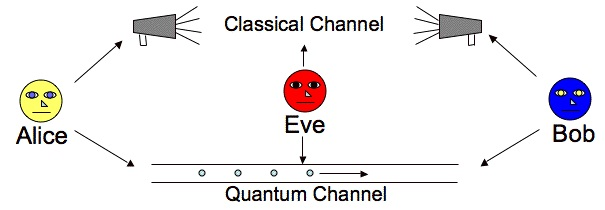
\includegraphics[scale=0.6]{imagenes/aeb}\\
	\end{center}
	Existe una forma mediante la cual Alice y Bob pueden acordar su clave secreta y, además, saber si hay alguien espiando sus comunicaciones.
\end{frame}

\begin{frame}
	\frametitle{Algunos experimentos. Distribución de Clave Cuántica}
	\begin{itemize}
	\item Alice quiere transmitir una clave binaria a Bob. Para ello utilizará el canal cuántico, que le permite enviar particulas cuánticas. Alice aleatoriamente utiliza para codificar cada bit una de estas dos bases: 
	$\filados{0\to\baseup}{1\to\baseright}$ o $\filados{0\to\baseupleft}{1\to\baseupright}$
	\item Bob recibe las partículas y por cada bit escoge una de las bases vistas previamente para medir. En el 50\% de las veces las bases escogidas por Alice y Bob coincidiran.
	\item A continuación Bob y Alice comunican qué bases escogieron por cada bit mediante el canal tradicional. La clave final de bits será la formada por los bits para los que Alice y Bob tomaron la misma base. \\ 
	\textbf{¿Pero qué pasa con Eve?}
	\end{itemize}
\end{frame}

\begin{frame}
	\frametitle{Algunos experimentos. Distribución de Clave Cuántica}
	\begin{itemize}
	\item Supongamos que Eve intercepta las partículas cuánticas, y realiza mediciones tomando de nuevo una base aleatoria de las vistas previamente. En un 50\% de las veces escogerá la base erronea y por tanto habrá proyectado la particula en dicha base, modificando su estado. 
	\item Cuando Bob reciba esta particula, en un 50\% de las veces habrá sido modificada por Eve, y por tanto a pesar de que acierte la base que escogió Alice para codificar el bit, hay otro 50\% de posibilidades de que el bit que mida sea erróneo. Es decir, en el 25\% de los bits, Alice y Bob habrán cogido la misma base y sin embargo sus medidas serán distintas! Sacando a luz así la existencia de una ``fuga'' en el canal cuántico.
	\end{itemize}
\end{frame}

\begin{frame}
	\frametitle{Algunos experimentos. Codificación Densa}
	\begin{itemize}
	\item Vamos a ver una forma de codificar 2 bits clásicos mediante un solo qubit. Para ello Alice y Bob deben poseer cada uno previamente una de las partículas de un par EPR ($\psi_0$) y el proceso que seguiremos será el siguiente:
	\begin{center}
	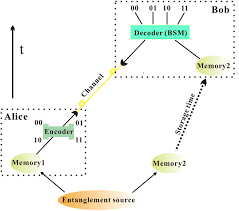
\includegraphics[scale=0.8]{imagenes/superdense}\\
	\end{center}
	\end{itemize}
\end{frame}

\begin{frame}
	\frametitle{Algunos experimentos. Codificación Densa}
	\begin{itemize}
	\item A continuación, Alice realiza las siguientes transformaciones sobre su qubit en función del valor que quiera codificar:
	
	\begin{center}
 		\begin{tabular}{||c c c||} 
 		\hline
 		Valor & Transformación & Nuevo Estado \\ [0.8ex] 
	 	\hline\hline
 		0 & $\psi_0 = (I \otimes I)\psi_0$ &  $\dfrac{1}{\sqrt{2}}(\base{00} + \base{11})$ \\ 
 		\hline
	 	1 & $\psi_1 = (X \otimes I)\psi_0$ &  $\dfrac{1}{\sqrt{2}}(\base{10} + \base{01})$  \\
 		\hline
	 	2 & $\psi_2 = (Y \otimes I)\psi_0$ &  $\dfrac{1}{\sqrt{2}}(-\base{10} + \base{01})$  \\
	 	\hline
	 	3 & $\psi_3 = (Z \otimes I)\psi_0$ &  $\dfrac{1}{\sqrt{2}}(\base{00} + -\base{11})$ \\[1ex]
	 	\hline
		\end{tabular}
	\end{center}
	\end{itemize}
\end{frame}

\begin{frame}
	\frametitle{Algunos experimentos. Codificación Densa}
	\begin{itemize}
	\item Bob recibe el qubit de Alice y realiza una Cnot sobre ambos bits, obteniendo las siguientes posibles resultados:
		\begin{center}
		\resizebox{\textwidth}{!}{%
 		\begin{tabular}{||c c c c||} 
 		\hline
 		Estado Inicial & CNot & Primer Bit & Segundo Bit\\ [0.4ex] 
	 	\hline\hline
 		$\psi_0 = \dfrac{1}{\sqrt{2}}(\base{00} + \base{11})$ & $\dfrac{1}{\sqrt{2}}(\base{00} + \base{10})$ &  $\dfrac{1}{\sqrt{2}}(\base0 + \base1)$ & $\base0$ \\ 
 		\hline
	 	$\psi_1 = \dfrac{1}{\sqrt{2}}(\base{10} + \base{01})$ & $\dfrac{1}{\sqrt{2}}(\base{11} + \base{01})$ & $\dfrac{1}{\sqrt{2}}(\base1 + \base0)$ & $\base1$ \\
 		\hline
	 	$\psi_2 = \dfrac{1}{\sqrt{2}}(-\base{10} + \base{01})$ & $\dfrac{1}{\sqrt{2}}(-\base{11} + \base{01})$ & $\dfrac{1}{\sqrt{2}}(-\base1 + \base0)$ & $\base1$ \\
	 	\hline
	 	$\psi_3 = \dfrac{1}{\sqrt{2}}(\base{00} + -\base{11})$ & $\dfrac{1}{\sqrt{2}}(\base{00} - \base{10})$ & $\dfrac{1}{\sqrt{2}}(\base0 - \base1)$ & $\base0$ \\[1ex]
	 	\hline
		\end{tabular}
		}
	\end{center}
	\item Ahora midiendo el segundo qubit, Bob ya puede saber si Alice a codificado un 0/3, o un 1/2.
	\end{itemize}
\end{frame}

\begin{frame}
	\frametitle{Algunos experimentos. Codificación Densa}
	\begin{itemize}
	\item Por último, Bob debe aplicar una Hadamard al primer bit. Es importante ver que las puertas Hadamard son matrices involutivas, es decir, inversas de sí mismas, por lo que obtenemos:
		\begin{center}
 		\begin{tabular}{||c c||} 
 		\hline
 		Primer Bit & Hadamard \\ [0.8ex] 
	 	\hline\hline
 		$\dfrac{1}{\sqrt{2}}(\base0 + \base1)$ & $\base0$ \\ 
 		\hline
		$\dfrac{1}{\sqrt{2}}(\base1 + \base0)$ & $\base0$ \\
 		\hline
		$\dfrac{1}{\sqrt{2}}(-\base1 + \base0)$ & $\base1$ \\
	 	\hline
	 	$\dfrac{1}{\sqrt{2}}(\base0 - \base1)$ & $\base1$ \\[1ex]
	 	\hline
		\end{tabular}
	\end{center}
	\item Y de esta forma Bob ya puede decodificar por completo 4 bits, habiendose producido la retransmisión de un solo qubit.
	\end{itemize}
\end{frame}

\begin{frame}
	\frametitle{Algunos experimentos. Teleportación}
	\begin{itemize}
	\item Ahora el objetivo es transmitir el estado cuántico de una partícula a traves de dos bits clásicos. Supongamos que Alice tiene un qubit del cual desconoce su estado: $\Phi = a\base0 + b\base1$.
	\item Y además, tanto Alice como Bob tienen un qubit de un par EPR ($\psi_0$). Por tanto el estado inicial viene dado por : \\ 
	\begin{center}
	$\Phi \otimes \psi_0 =  (a\base0 + b\base1) \otimes\dfrac{1}{\sqrt{2}}(\base{00} + \base{11}) = \dfrac{1}{\sqrt{2}} (a\base{000} + a\base{011} + b\base{100} + b\base{111}$
	\end{center}
	\end{itemize}
\end{frame}

\begin{frame}
	\frametitle{Algunos experimentos. Teleportación}
	\begin{itemize}
	\item Ahora Alice realiza las siguientes transformaciones sobre los dos primeros qubits (coinciden con el paso de decodificación en el experimento de Codificación Densa):
	\begin{center}
	$ (H \otimes I \otimes I)(\cnot \otimes I) (\Phi \otimes \psi_0) = ... = \dfrac{1}{2}(\base{00}(a\base0 + b\base1) + \base{01}(a\base1 + b\base0) + \base{10}(a\base0 - b\base1) + 
	\base{11}(a\base1 - b\base0)) $ 
	\end{center}
	\item Por tanto si Alice mide los dos primeros qubits, tiene la misma probabilidad de medir $\base{00}, \base{10}, \base{01} o \base{11}$. Alice transfiere el resultado de su medición mediante 		dos bits clásicos.
	\end{itemize}
\end{frame}

\begin{frame}
	\frametitle{Algunos experimentos. Teleportación}
	\begin{itemize}
	\item En función de la medición realizada por Alice, el qubit de Bob se ve proyectado de la siguientes formas, y por tanto podemos aplicar transformaciones para recuperar el qubit inicial  $\Phi$:
	\begin{center}
 		\begin{tabular}{||c c c||} 
 		\hline
 		Bits Recibidos & Estado Tercer Qubit & Transformación \\ [0.8ex] 
	 	\hline\hline
 		00 & $a\base0 + b\base1$ & I \\ 
 		\hline
	 	01 & $a\base1 + b\base0$ & X \\
 		\hline
	 	10 & $a\base0 - b\base1$ & Z \\
	 	\hline
	 	11 & $a\base1 - b\base0$ & Y \\[1ex]
	 	\hline
		\end{tabular}
	\end{center}
	\item Es importante ver que no violamos la propiedad de no-clonación, pues el estado inicial del qubit de Alice se ha perdido al realizar una medición sobre este.
	\end{itemize}
\end{frame}

\section{Computación Cuántica}

\begin{frame}
	\frametitle{Computación Cuántica. \textit{Gatearray} cuántico}
	Como ya hemos visto, las puertas cuánticas deben ser reversibles; Sin embargo, muchos operadores clásicos como AND, OR o NAND no lo son. Veamos cómo podemos solucionar este problema.\newline
	
	\begin{Large}\textbf{La puerta \textit{Toffoli}}\end{Large}
	\newline\\
	La puerta not controlada de 3 bits o puerta \textit{Toffoli} viene dada por la notación:
	$T=\base0\lbase0\otimes I\otimes I +\base1\lbase1\otimes \cnot=$
	$\left({\begin{array}{c|c}	I_4&0\\\hline0&\cnot \end{array} } \right)$. Tenemos:
	
	\begin{itemize}
	\item $T\base{1,1,x}=\base{1,1,\neg x}\equiv$ NOT clásica
	\item $T\base{x,y,0}=\base{x,y,x\land y}\equiv$ AND clásica
	\end{itemize}
	Puesto que AND y NOT es un \textbf{conjunto lógico funcionalmente completo}, la puerta $T$ es suficiente para construir cualquier circuito arbitrario.
\end{frame}

\begin{frame}
	\frametitle{Computación Cuántica. \textit{Gatearray} cuántico}
	\begin{block}{Sumador}
	En la figura de abajo mostramos un sumador de un bit. $x$ e $y$ son los bits a sumar, $c$ el acarreo entrante, $s$ la suma y $c'$ el acarreo saliente.
	\end{block}
	\begin{center}
	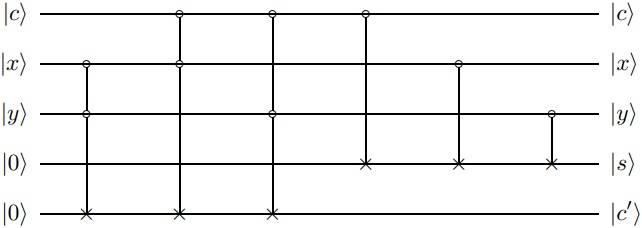
\includegraphics[scale=0.5]{imagenes/sumador}
	\end{center}
\end{frame}

\begin{frame}
	\frametitle{Computación Cuántica. \textit{Gatearray} cuántico}
	\begin{itemize}
	\item En 1985 \textit{Deutsch} probó que es posible construir puertas clásicas reversibles para cualquier función clásica computable.
	\item En 1997 \textit{Bernstein} y \textit{Vazirani} prueban que de hecho se puede concebir como una máquina de \textit{Turing} cuántica.
	\item Es decir, para cualquier función $f$ clásica con $m$ bits de entrada y $k$ bits de salida puede ser implementada en un computador cuántico.
	\item Denotamos a dicha implementación $U_f$ como \textbf{\textit{gatearray} cuántico} que no es más que una transformación de $m+k$ qubits de forma $U_f:\base{x,y}\to\base{x,y\oplus$\footnote{$\oplus$ denota la operación XOR}$f(x)}$
	\item para computar $f(x)$ basta con aplicar $U_f$ a $\base{x}\otimes\base{\overset{k}{00\hdots0}}$ que denotamos como $\base{x,0}$. Además, como $f(x)\oplus f(x) = 0$, tenemos que $U_fU_f=I$.
	\end{itemize}
\end{frame}

\begin{frame}
	\frametitle{Computación Cuántica. Paralelismo}
	\begin{itemize}
	\item ¿Qué pasa si utilizando puertas de \textit{Hadamard} conseguimos una superposición de estados y lo utilizamos como entrada para $U_f$? En resumidas cuentas, que obtenemos una superposición con todos los resultados en un único cómputo.
	\item Por ejemplo, apliquemos una puerta de \textit{Toffoli} al estado inicial $H\base0\otimes H\base0\otimes 0 = \frac{1}{2}(\base{000}+\base{010}+\base{100}+\base{110})$ (recordemos que $T\base{x,y,0}=\base{x,y,x\land y}$).
	\item Luego $T(H\base0\otimes H\base0\otimes 0)=\frac{1}{2}(\base{000}+\base{010}+\base{100}+\base{111})$. Como los valores $x$, $y$ y $x\land y$ están entrelazados es indiferente el orden en qué midamos.
	\item El problema es que al medir sólo conseguiremos un único par de valores entrada y salida. Así que no hemos conseguido ningún ventaja adicional con respecto a un computador clásico y además, en este caso, no hemos podido elegir qué resultado medir.
	\end{itemize}
\end{frame}

\begin{frame}
	\frametitle{Algoritmo de búsqueda de \textit{Grover}}
	\begin{itemize}
	\item Sin embargo, podremos aprovechar este paralelismo con el uso de técnicas (sin analogía con a la programación clásica) que hagan que las medidas de los resultados deseados sean más probables de obtener.
	\item Supongamos que tenemos una lista no ordenada de tamaño \textbf{N} y sea $n$ tal que $2^n \geqslant N$ . Queremos buscar una entrada $x$ que verifica cierta propiedad $P$.
	\item Sea $U_p$ la puerta cuántica que implementa la función clásica $P(x)$ que devuelve 1 cuando $x$ cumple la propiedad. Por tanto tenemos:
	\begin{center}
		$U_p : \base{x,0} \to  \base{x,P(x)}$
	\end{center}
	\end{itemize}
\end{frame}

\begin{frame}
	\frametitle{Algoritmo de búsqueda de \textit{Grover}}
	El algoritmo de \textit{Grover} consta de los siguiente pasos:
	\begin{enumerate}
	\item Preparar una superposición de los $2^n$ posibles valores de entrada $x_i$.
	\item Aplicar la puerta $U_p$ a dicho estado, obteniendo: 
		\begin{center}
		$\dfrac{1}{\sqrt{2^n}} \sum_{i=0}^{2^n - 1}\base{x_i,P(x_i)}$
		\end{center}
	\item Cambiar la amplitud $a_j \to -a_j$ para cada $x_j$ tal que $P(x_j) = 1$.
	\item Realizar inversión sobre la media, incrementando la amplitud de los $x_j$ tales que $P(x_j) = 1$, y disminuyendo la de aquellos tales que $P(x_i) = 0$. \\
	Repetir los pasos \textbf{2-4} $\frac{\pi}{4}\sqrt{2^n}$ veces.
	\end{enumerate}
\end{frame}

\begin{frame}
	\frametitle{Algoritmo de búsqueda de \textit{Grover}}
	\begin{itemize}
	\item En 1996  \textit{Boyer} mostró que tras $\frac{\pi}{8}\sqrt{2^n}$ iteraciones la tasa de error es de 0,5. Sin embargo, tras $\frac{\pi}{4}\sqrt{2^n}$ iteraciones esta tasa baja hasta $2^{-n}$.
	\item Sin embargo, si seguimos aumentando el número de iteraciones los resultados empeoran. Esto se debe a que las transformaciones unitarias no son más que rotaciones en el espacio complejo y al rotar una solución muy próxima, podemos alejarnos.
	\end{itemize}
\end{frame}

\begin{frame}
	\frametitle{Algoritmo de búsqueda de \textit{Grover}}
	Ejemplo en Qiskit para una lista de tamaño 8. Los estados a buscar son $\base{101}$ y $\base{110}$.\\
	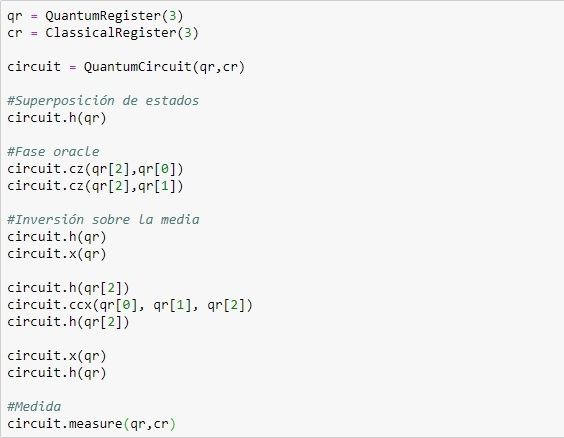
\includegraphics[scale=0.58]{imagenes/grovercodigo}
\end{frame}

\begin{frame}
	\frametitle{Algoritmo de búsqueda de \textit{Grover}}
	Circuito generado por el código.
	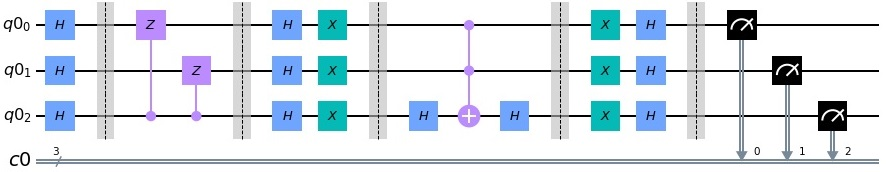
\includegraphics[scale=0.525]{imagenes/grovercircuito}
\end{frame}

\begin{frame}
	\frametitle{Algoritmo de búsqueda de \textit{Grover}}
	Resultados en simulador tras 1024 ejecuciones.
	\begin{center}
	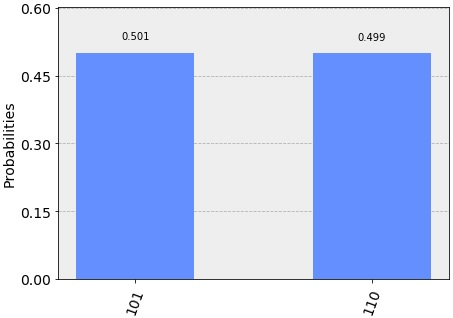
\includegraphics[scale=0.7]{imagenes/groverresultados}
	\end{center}
	513 veces se saldó con la medición \textbf{101}, mientras que 510 lo hizo con \textbf{110}.
\end{frame}



\end{document}
